
%(BEGIN_QUESTION)
% Copyright 2010, Tony R. Kuphaldt, released under the Creative Commons Attribution License (v 1.0)
% This means you may do almost anything with this work of mine, so long as you give me proper credit

Identifiser hvordan \textit{forsterkningen} til denne pneumatisk proporsjonalregulatoren vil endres hvis utgangsbelgen erstattes med en belg som har mindre areal for trykket å virke på:

$$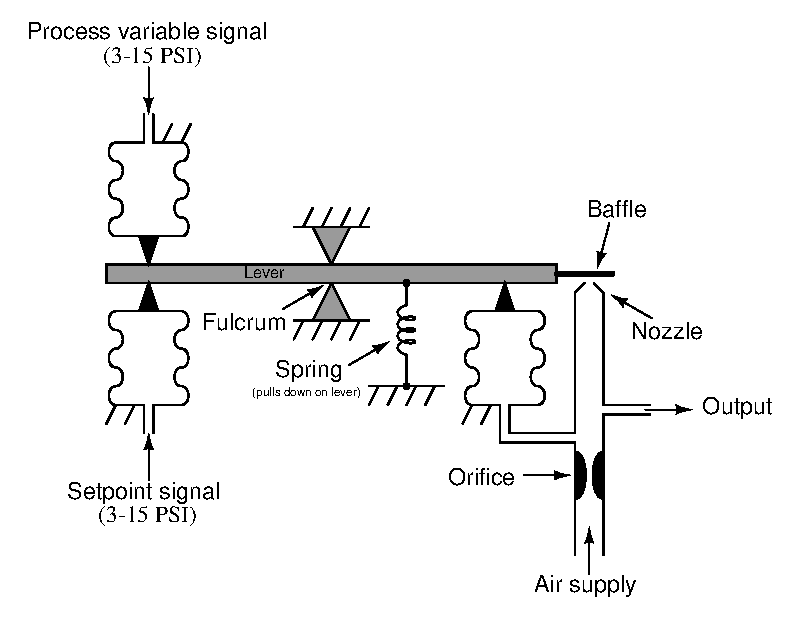
\includegraphics[width=15.5cm]{i00165x01.eps}$$

Angi om regulatorforsterkningen vil \textit{øke}, \textit{reduseres} eller \textit{forbli uendret}.

\vskip 30pt

\underbar{file i00165}
%(END_QUESTION)





%(BEGIN_ANSWER)

Forsterkningen vil {\bf øke} hvis utgangsbelgen gjøres mindre.

%(END_ANSWER)





%(BEGIN_NOTES)

{\bf This question is intended for exams only and not worksheets!}.

%(END_NOTES)

